\documentclass[tikz,border=0pt,11pt]{standalone}
\usepackage[T1]{fontenc}
\usepackage[utf8]{inputenc}
\usepackage{lmodern,amsmath,amssymb}
\usepackage[swedish]{babel}
\usetikzlibrary{arrows.meta,calc,positioning,decorations.pathmorphing,decorations.pathreplacing,patterns,shadings}
\definecolor{navy}{HTML}{102F40}
\definecolor{teal}{HTML}{147D78}
\definecolor{lightteal}{HTML}{E6F1ED}
\definecolor{gold}{HTML}{B88B3B}
\definecolor{palegold}{HTML}{F7EEDB}
\definecolor{rust}{HTML}{B6533B}
\definecolor{palerust}{HTML}{FAEAE4}
\definecolor{paper}{HTML}{F7F5EE}
\definecolor{muted}{HTML}{5B6D72}
\definecolor{line}{HTML}{D6DED8}
\renewcommand{\familydefault}{\sfdefault}
\newcommand{\atom}[5]{\shade[ball color=#3!70] (#1,#2) circle (#5);\node[text=white,font=\bfseries\small] at (#1,#2){#4};}
\newcommand{\water}[3]{\begin{scope}[shift={(#1,#2)},scale=#3]\draw[navy!45,line width=2pt] (-.3,.22)--(0,0)--(.3,.22);\atom{0}{0}{rust}{O}{.22}\atom{-.3}{.22}{teal}{H}{.15}\atom{.3}{.22}{teal}{H}{.15}\end{scope}}
\newcommand{\panel}[4]{\filldraw[fill=white,draw=line,rounded corners=5pt] (#1,#2) rectangle ++(#3,#4);}
\newcommand{\note}[4]{\node[txt,text width=#3cm] at (#1,#2){#4};}
\tikzset{txt/.style={anchor=north west,align=left,text=navy,font=\small},
 head/.style={anchor=west,text=navy,font=\bfseries\large},
 label/.style={align=center,text=navy,font=\small},
 smalllabel/.style={align=center,text=muted,font=\footnotesize},
 arrow/.style={-{Latex[length=2.5mm,width=1.8mm]},line width=1.2pt,draw=teal},
 goldarrow/.style={-{Latex[length=2.5mm]},line width=1.2pt,draw=gold},
 rustarrow/.style={-{Latex[length=2.5mm]},line width=1.2pt,draw=rust},
 dashedarrow/.style={arrow,dashed},
 badge/.style={fill=lightteal,rounded corners=3pt,text=teal,font=\bfseries\small,inner sep=5pt}}
\begin{document}
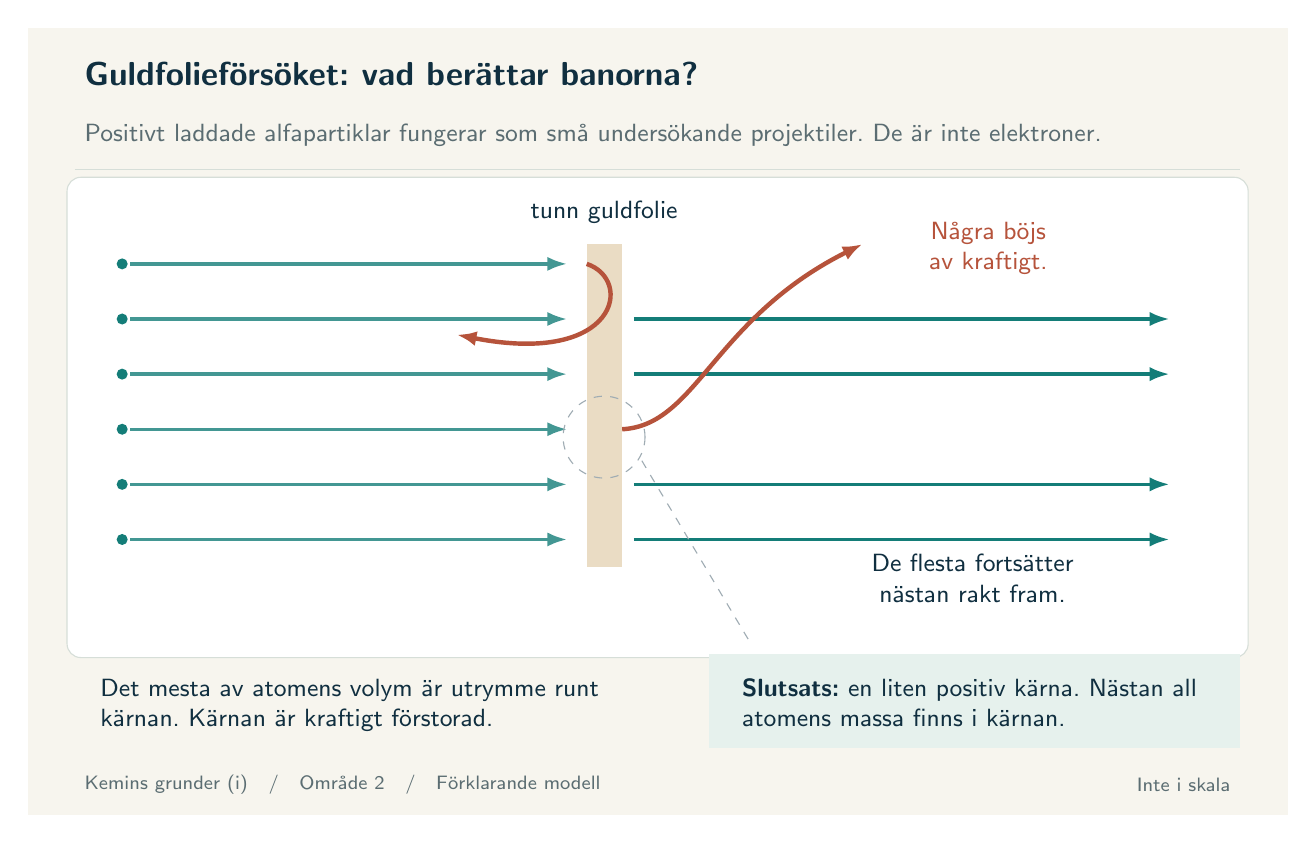
\begin{tikzpicture}[x=1cm,y=1cm]
\path[use as bounding box] (0,0) rectangle (16,10);
\fill[paper] (0,0) rectangle (16,10);
\node[head] at (.6,9.4){Guldfolieförsöket: vad berättar banorna?};
\note{.6}{8.9}{14.8}{\textcolor{muted}{Positivt laddade alfapartiklar fungerar som små undersökande projektiler. De är inte elektroner.}}
\draw[line] (.6,8.2)--(15.4,8.2);

\panel{.5}{2}{15}{6.1}
\fill[gold!30] (7.1,3.15) rectangle(7.55,7.25);\node[label] at (7.32,7.65){tunn guldfolie};
\foreach \y in {3.5,4.2,4.9,5.6,6.3,7}{\draw[arrow,teal!80] (1.3,\y)--(6.85,\y);\fill[teal] (1.2,\y) circle(.07);}
\foreach \y in {3.5,4.2,5.6,6.3}{\draw[arrow] (7.7,\y)--(14.5,\y);}
\draw[rustarrow,line width=1.6pt] (7.55,4.9).. controls (8.5,4.95) and (8.7,6.3)..(10.6,7.25);
\draw[rustarrow,line width=1.6pt] (7.1,7).. controls (7.7,6.8) and (7.5,5.7)..(5.45,6.1);
\node[label,text width=4cm] at (12,3){De flesta fortsätter nästan rakt fram.};
\node[label,text width=3cm,text=rust] at (12.2,7.2){Några böjs av kraftigt.};
\draw[dashed,navy!40] (7.32,4.8) circle(.52);\draw[dashed,navy!40] (7.8,4.5)--(9.2,2.15);
\fill[lightteal] (8.65,.85) rectangle(15.4,2.05);

\node[txt,text width=6.1cm] at (8.95,1.85){\textbf{Slutsats:} en liten positiv kärna. Nästan all atomens massa finns i kärnan.};
\node[txt,text width=7.1cm] at (.8,1.85){Det mesta av atomens volym är utrymme runt kärnan. Kärnan är kraftigt förstorad.};\node[anchor=west,text=muted,font=\scriptsize] at (.6,.38){Kemins grunder (i)\quad /\quad Område 2\quad /\quad Förklarande modell};
\node[anchor=east,text=muted,font=\scriptsize] at (15.4,.38){Inte i skala};
\end{tikzpicture}\end{document}
